% -*- TeX-master: "main.tex" -*-

% "Stand der Technik" (Was gibt es schon?)
\chapter{Existing APIs}
\label{ch:existing}
\label{unsuitable}

Other browsers (such as Firefox or Chrome) have been supporting extensions for a
long time. When designing an extension API, it is useful to understand this
previous work. It can serve as an inspiration, in order to follow common standards and learn
from mistakes made in the past. Therefore, various existing extension APIs have
been analyzed.

\section{Firefox XUL extension API}

Older versions of the Firefox web browser used to have a very powerful extension
API, based on its XUL (XML User Interface Language) technology. However, this
approach presented various challenges and was thus recently abandoned, while
adopting the WebExtensions standard.

The apparent philosophy behind ``legacy'' Firefox addons was to allow maximum
customizability from extensions -- however, this came with various drawbacks
which ultimately led to Mozilla abandoning that approach.

The motivations to deprecate and subsequently remove the legacy addon API listed
in Mozilla's blog post \autocite{mozilla-webext} were as follows:

\begin{itemize}
  \item Chrome and Opera (and nowadays also Microsoft Edge) already supported
    the WebExtension API, so a switch to the WebExtension API would drastically
    reduce the effort required for developers when implementing extensions with
    cross-browser compatibility: \emph{``We would like add-on development to be more
    like Web development: the same code should run in multiple browsers according to
    behavior set by standards, with comprehensive documentation available from
    multiple vendors.''}
  \item Firefox' Electrolysis (e10s)
    project\footnote{\url{https://wiki.mozilla.org/Electrolysis}} was a big
    change in its codebase, with the goal of separating tabs into separate
    processes, for security and performance reasons. Many legacy addons were not
    compatible with the changes necessary for Electrolysis. This forced either
    the add-on developer to make (sometimes intricate) changes to their code; or
    the user's Firefox instance to run in a special fallback mode: \emph{``Add-ons
    that haven't been upgraded to work with Electrolysis will run in a special
    compatibility environment that resembles single-process Firefox as much as
    possible. [...] However, [the fallback is] much slower than the equivalent DOM
    operations in single-process Firefox, and can affect the user experience
    negatively. Also, some accesses aren't supported by the compatibility layer and
    will throw exceptions.''}
  \item Since Firefox is a quite popular product, malicious Firefox addons
    started to become an attractive attack vector for bad actors. With legacy
    addons, addon code is able to run arbitrary code and freely modify Firefox
    internals on the user's machine, which turns untrusted addons into a
    security liability \autocite{mozilla-signing}.
  \item Legacy addons hindered Firefox development in general, since its
    powerful addon API introduced a tight coupling between Firefox' internal
    code, and the code in third-party addons: \emph{``A permissive add-on model
    means that we have limited flexibility in changing the foundations of Firefox.
    [...] Without a fundamental shift to the way Firefox add-ons work, we will
    be unable to use new technologies like Electrolysis, Servo\footnote{An
      experimental new rendering engine by Mozilla, implemented in the Rust
      programming language. Parts of Servo (such as its CSS renderer) have since
    been merged into Firefox.} or browser.html\footnote{A Mozilla research
    project which implements a browser completely in HTML, now retired.}
    as part of Firefox. The tight coupling between the browser and its add-ons
    also creates shorter-term problems for Firefox development. It's not uncommon
    for Firefox development to be delayed because of broken add-ons.''}
\end{itemize}

While qutebrowser should learn from the mistakes made in Firefox' legacy API,
a more thorough analysis of the XUL API design proved to be difficult. Archived
API documentation is still
available\footnote{\url{https://developer.mozilla.org/en-US/docs/Archive/Add-ons}},
but bad documentation was one of the criticisms of XUL addons
\autocite{mozilla-webext}. Since the API is not in active use anymore, and ties
into Firefox' core code deeply, no further analysis was performed.

The key takeaway for qutebrowser is that it should have a minimal and clearly
outlined extension API, rather than naively exposing its internal Python code to
extensions.

\section{WebExtensions API}
\label{webextensions}

Currently, there are ongoing efforts towards a \emph{WebExtensions} API for browser
extensions, which is shared between different
browsers. WebExtensions are supported by Chrome, Opera, Firefox and Edge.
Efforts are currently underway to standardize the API as a W3C specification
\autocite{w3c-webext}. At the moment, each browser has a slightly different set of
supported APIs, with some divergence in naming. As an example, the
\verb|chrome.| module is used in Chromium for browser-specific features, while
Firefox uses \verb|browser.|.

If qutebrowser supported the WebExtension API, it would follow a common
standard, and enable running thousands of existing Chromium extensions with
little to no adjustment to their code.

Unfortunately, WebExtensions are unsuitable for qutebrowser, for various
reasons:

\begin{itemize}
  \item Full WebExtension support would likely require some degree of support by
    the underlying rendering engine. While there is an open
    suggestion\footnote{\url{https://bugreports.qt.io/browse/QTBUG-61676}} in
    Qt's bug tracker, no work on that has been started so far.
  \item Implementing WebExtension support in Python only (without any support
    from the underlying backend) is hard, if possible at all. Neither
    backend allows deep access to its JavaScript engine
    (V8\footnote{\url{https://v8.dev/}} for QtWebEngine, JavaScriptCore for
    QtWebKit), which means extension code would have to run in a separate
    JavaScript interpreter (such as Qt's
    \verb|QJSEngine|\footnote{\url{http://doc.qt.io/qt-5/qjsengine.html}} class).
    However, extensions should have access to web contents. Thus, a secure
    communication channel is needed between the backend's JavaScript interpreter
    (used for the page), and the separate interpreter used for extensions. In
    addition, it should only be possible for extensions to access page content,
    not the other way around, as that would be a security issue. All in all,
    this approach is prohibitively complex, and thus out of scope for this SA.
  \item Most qutebrowser users and contributors are accustomed to writing Python
    code (since qutebrowser itself is written in Python). While a WebExtension
    API (in JavaScript) would allow using thousands of existing Chrome extensions, a
    Python API will make it easier for users to write custom additions to
    qutebrowser to suit their needs.
  \item The security model of WebExtensions is fundamentally different from
    what is intended for qutebrowser extensions -- WebExtension code is sandboxed,
    and unable to run arbitrary code on the user's machine. This can be worked
around by using WebExtension's ``native
    messaging''\footnote{\url{https://developer.mozilla.org/en-US/docs/Mozilla/Add-ons/WebExtensions/Native_messaging}}
    capability with a separate application running in the background, but doing
    so is cumbersome. See \ref{security} for an explanation on the security
    model of qutebrowser extensions.
  \item The WebExtension API was not designed with the Qt APIs in mind, yet
    qutebrowser is bound to using those. In some cases it might be possible to
    write an adapter to bring the two approaches together; but if they are
    fundamentally different, doing so might prove difficult. With a custom API,
    there is more control over the tradeoff between an API which closely follows
    Qt's (and thus reduces friction and complexity), or an API which prioritizes
    other considerations (see \ref{criteria}).
\end{itemize}

While it is not possible for qutebrowser to implement support for WebExtensions,
they are still useful as a source for API design inspiration. However, it
should be noted that the WebExtension API is closely tied to the JavaScript
language, so architecture decisions taken there will not necessarily be
applicable to qutebrowser's Python extension API.

\subsection{Anatomy of a WebExtension}
\label{anatomy}

As explained in Mozilla's
documentation\footnote{\url{https://developer.mozilla.org/en-US/docs/Mozilla/Add-ons/WebExtensions/Anatomy_of_a_WebExtension},
  accessed 2018-11-08},
a WebExtension consists of various files:

\begin{itemize}
  \item A \verb|manifest.json| manifest file, which lists meta information about
    an extension, such as its name, its author, or the permissions it requests.
  \item Background scripts, which are used to implement long-running operations.
    An extension's background scripts are loaded for the entire lifetime of an
    extension, i.e., until it is disabled or uninstalled.
  \item Content scripts, which are injected into loaded web pages, and can
    interact with their content (access and manipulate the DOM). They also have
    some additional permissions, which scripts supplied by the page do not have,
    such as messaging with an extension's background scripts.
  \item HTML pages for user interfaces such as an extension's option page or sidebar.
  \item Other resources such as icons.
\end{itemize}

These files are then packaged into a specially named ZIP file (XPI in case of
Firefox; CRX for Chromium) and distributed via an extension store (a special
website run by Mozilla/Google).

For qutebrowser extensions, a simpler approach will be taken: Extensions can
consist of a single standalone \verb|.py| file which implements the necessary
functionality. This mechanism is inspired by the plugin handling of the pytest
project\footnote{\url{https://docs.pytest.org/en/latest/writing_plugins.html},
  accessed 2018-11-08}. In the future, this makes it trivial for users to add
their own extensions to qutebrowser. That solution is also very straightforward and
appropriate for the initial goal of refactoring qutebrowser's core code into
extensions.

Due to extensions being written in Python, the above separation between content
and background scripts also does not fully apply to qutebrowser's API. The Python
extensions can be seen as a background script.

\subsection{Analysis of the WebExtension API}

The WebExtensions API is separated into various modules, each of which is
briefly analyzed in the context of qutebrowser in this section, sorted
alphabetically. The indented descriptions are copied verbatim from Mozilla's API
documentation\footnote{\url{https://developer.mozilla.org/en-US/docs/Mozilla/Add-ons/WebExtensions/API},
  \\ accessed 2018-11-02}.

\subsubsection{alarms}
\begin{quote}
Schedule code to run at a specific time in the future.
\end{quote}

Since qutebrowser extensions will have access to the Qt GUI library, no
equivalent to this module is needed. Qt provides the
\verb|QTimer|\footnote{\url{http://doc.qt.io/qt-5/qtimer.html}} class, which can
be used for equivalent functionality.

\subsubsection{bookmarks}
\begin{quote}
The WebExtensions bookmarks API lets an extension interact with and manipulate the browser's bookmarking system. You can use it to bookmark pages, retrieve existing bookmarks, and edit, remove, and organize bookmarks.
\end{quote}

Bookmarks in qutebrowser are currently much simpler than they are in Firefox or
Chrome; i.e. they are not organized in a tree-like structure, and features like
tags are missing. Therefore, the bookmarks WebExtension API does not fit well
with qutebrowser bookmarks.

There is an ongoing
contribution\footnote{\url{https://github.com/qutebrowser/qutebrowser/pull/3855}}
to add such features, and it would make little sense to add an extension API before
that contribution is merged. Since access to bookmarks is not vital for an extension
API, it is currently out of scope.

\subsubsection{browserAction, menus, pageAction, sidebarAction}
\begin{quote}
browserAction: Adds a button to the browser's toolbar.
\end{quote}
\begin{quote}
menus: Add items to the browser's menu system.
\end{quote}
\begin{quote}
pageAction: A page action is a clickable icon inside the browser's address bar.
\end{quote}
\begin{quote}
sidebarAction: Gets and sets properties of an extension's sidebar.
\end{quote}

These modules allow extensions to add their own user interface elements to the
browser, as shown in figure \ref{img:browser-action}.

\begin{figure}[h]
  \centering
  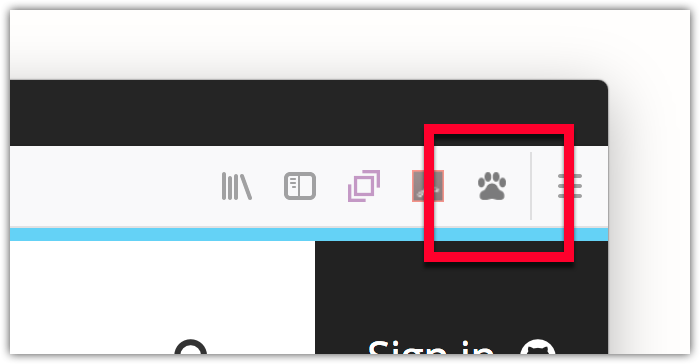
\includegraphics[width=0.5\linewidth]{img/browser-action.png}
  \caption{A button added via the \texttt{browserAction} WebExtension API}
  \label{img:browser-action}
\end{figure}

It should be possible for custom qutebrowser extensions to add their own user
interface elements. However, this functionality is unlikely to be needed
when moving core functionality into extensions (which is the main focus of this
SA). Therefore, this API is currently out of scope.

\subsubsection{browserSettings}
\begin{quote}
Enables an extension to modify certain global browser settings.
\end{quote}

Extensions for qutebrowser should be able to modify its settings, and also
define their own options.

\subsubsection{browsingData}
\begin{quote}
Enables extensions to clear the data that is accumulated while the user is
browsing.
\end{quote}

No such functionality is currently implemented in qutebrowser, so this API is
out of scope.

\subsubsection{clipboard}
\begin{quote}
The clipboard API enables an extension to copy items to the system clipboard.
\end{quote}

Since qutebrowser extensions will have access to the Qt GUI library, no
equivalent to this module is needed. Qt provides the
\verb|QClipboard|\footnote{\url{http://doc.qt.io/qt-5/qclipboard.html}} class, which can
be used for equivalent functionality.

\subsubsection{commands}
\begin{quote}
Listen for the user executing commands that you have registered using the commands manifest.json key.
\end{quote}

This API is used to register custom keyboard shortcuts in WebExtensions. A
similar concept also exists in qutebrowser, where commands can either be bound
to keys (using the configuration), or executed in the commandline via \verb|:command|.

This API is important, since many core parts register commands in qutebrowser
(like \verb|:adblock-update| for the ad blocker). Thus, Extensions should be
able to register Python functions as commands.

\subsubsection{contentScripts}
\begin{quote}
With the contentScripts API, an extension can register and unregister scripts at runtime.
\end{quote}

Injecting custom JavaScript code into websites will be an useful feature for
custom extensions at a later stage, but is not needed to move code out of
qutebrowser's core, as it is expected for internal JavaScript code to stay in the
core part. Thus, this module is currently out of scope.

Running JavaScript one-off snippets (triggered manually, rather than
automatically on page load) is already implemented in the tab API, and should be
trivial to expose to extensions.

\subsubsection{contextualIdentities, i18n, identity, idle, notifications, pkcs11, topSites}
\begin{quote}
contextualidentities: Work with contextual identities: list, create, remove, and update contextual identities.
\end{quote}
\begin{quote}
i18n: Functions to internationalize your extension. You can use these APIs to get localized strings from locale files packaged with your extension, find out the browser's current language, and find out the value of its Accept-Language header.
\end{quote}
\begin{quote}
identity: Use the identity API to get an OAuth2 authorization code or access token, which an extension can then use to access user data from a service which supports OAuth2 access (such as a Google or a Facebook account).
\end{quote}
\begin{quote}
idle: Find out when the user's system is idle, locked, or active.
\end{quote}
\begin{quote}
notifications: Display notifications to the user, using the underlying operating system's notification mechanism.
\end{quote}
\begin{quote}
pkcs11: The pkcs11 API enables an extension to enumerate PKCS\#11 security modules, and to make them accessible to the browser as sources of keys and certificates.
\end{quote}
\begin{quote}
topSites: Use the topSites API to get an array containing pages that the user has visited often and frequently.
\end{quote}

No such functionality is currently implemented in qutebrowser, so the above
modules are out of scope.

\subsubsection{cookies}
\begin{quote}
Enables extensions to get and set cookies, and be notified when they change.
\end{quote}

Cookie access is not fully exposed by the QtWebEngine
library\footnote{\url{http://doc.qt.io/qt-5/qwebenginecookiestore.html}}, so
it is currently impossible to implement this module.

\subsubsection{devtools}
\begin{quote}
The devtools.inspectedWindow API lets a devtools extension interact with the window that the developer tools are attached to.
\end{quote}

\begin{quote}
The devtools.network API lets a devtools extension get information about network requests associated with the window that the devtools are attached to (the inspected window).
\end{quote}

\begin{quote}
The devtools.panels API lets a devtools extension define its user interface inside the devtools window.
\end{quote}

Access to developer tools is not exposed by the QtWebEngine library, so it is
currently impossible to implement this module.

\subsubsection{dns}
\begin{quote}
Enables an extension to resolve domain names.
\end{quote}

Since qutebrowser extensions will have access to the Qt GUI library, no
equivalent to this module is needed. Qt provides the
\verb|QDnsLookup|\footnote{\url{http://doc.qt.io/qt-5/qdnslookup.html}} class, which can
be used for equivalent functionality.

\subsubsection{downloads}
\begin{quote}
Enables extensions to interact with the browser's download manager. You can use this API module to download files, cancel, pause, resume downloads, and show downloaded files in the file manager.
\end{quote}

This module is needed for various core parts (such as the ad blocker, to
download filter lists).

\subsubsection{events, extensions, extensionTypes, permissions, runtime, types}
\begin{quote}
events: Common types used by APIs that dispatch events.
\end{quote}
\begin{quote}
extensions: Utilities related to your extension. Get URLs to resources packages with your extension, get the Window object for your extension's pages, get the values for various settings. Note that the messaging APIs in this module are deprecated in favor of the equivalent APIs in the runtime module.
\end{quote}
\begin{quote}
extensionTypes: Some common types used in other WebExtension APIs.
\end{quote}
\begin{quote}
permissions: Extensions need permissions to access more powerful WebExtension APIs. They can ask for permissions at install time, by including the permissions they need in the permissions manifest.json key. The main advantages of asking for permissions at install time are:
\end{quote}
\begin{quote}
runtime: This module provides information about your extension and the environment it's running in.
\end{quote}
\begin{quote}
types: Defines the BrowserSetting type, which is used to represent a browser setting.
\end{quote}

The above APIs are specific to the WebExtensions API, and thus irrelevant for
qutebrowser.

\subsubsection{find}
\begin{quote}
Finds text in a web page, and highlights matches.
\end{quote}

This functionality is already available as part of qutebrowser's tab API (see
section \ref{tabapi}), and should be trivial to expose to extensions.

\subsubsection{history}
\begin{quote}
Use the history API to interact with the browser history.
\end{quote}

Accessing and manipulating the history might be an useful feature for future
user-contributed extensions, but is likely not needed for moving code out of
qutebrowser's core. Thus, the history module is currently out of scope.

\subsubsection{management}
\begin{quote}
Get information about installed add-ons.
\end{quote}

Extensions are currently not expected to interact with each other (even less so
when moving code out of the core), so this module is not needed.

\subsubsection{omnibox}
\begin{quote}
Enables extensions to implement customised behavior when the user types into the
browser's address bar.
\end{quote}

When adding custom commands, extensions also should be able to specify a
completion function, so users can use qutebrowser's autocompletion when typing
the extension's commands.

\subsubsection{privacy}
\begin{quote}
Access and modify various privacy-related browser settings.
\end{quote}

In qutebrowser, these settings (like
\verb|privacy.network.webRTCIPHandlingPolicy|) are exposed as normal qutebrowser
settings (like \verb|content.webrtc_ip_handling_policy|), so there is no need
for a similar module in the extension API.

\subsubsection{proxy}
\begin{quote}
Use the proxy API to proxy web requests. There are two different ways you can do this:
\end{quote}

No low-level networking access is possible via the QtWebEngine API, so this
module will not be implemented.

\subsubsection{search}
\begin{quote}
Retrieves search engines and executes a search with a specific search engine.
\end{quote}

Search engines are part of the main configuration in qutebrowser, so an
extension can trivially retrieve a search engine from there and execute a query
without the need for a dedicated API.

\subsubsection{sessions}
\begin{quote}
Use the sessions API to list, and restore, tabs and windows that have been closed while the browser has been running.
\end{quote}

While qutebrowser does have a session feature, access to it is not vital for an
extension API, so this is currently out of scope.

\subsubsection{storage}
\begin{quote}
Enables extensions to store and retrieve data, and listen for changes to stored items.
\end{quote}

Having a simple way to persist data for extensions will be an useful feature for
third-party extensions, but is currently not needed when moving code out of the core.

\subsubsection{tabs, windows}
\begin{quote}
tabs: Interact with the browser's tab system.
\end{quote}
\begin{quote}
windows: Interact with browser windows. You can use this API to get information about open windows and to open, modify, and close windows. You can also listen for window open, close, and activate events.
\end{quote}

Various functionality already exists in qutebrowser as part of the ``tab API''
(documented in section \ref{tabapi}), which should be trivial to expose to the
extension API. Furthermore, the \verb|tabs| and \verb|windows| modules contains
various functionality to retrieve tabs, which should be added to qutebrowser's
extension API.

\subsubsection{theme}
\begin{quote}
Enables browser extensions to update the browser theme.
\end{quote}

No dedicated theme feature exists in qutebrowser - instead, qutebrowser's user
interface can be customized using its configuration.

\subsubsection{webNavigation}
\begin{quote}
Add event listeners for the various stages of a navigation. A navigation consists of a frame in the browser transitioning from one URL to another, usually (but not always) in response to a user action like clicking a link or entering a URL in the location bar.
\end{quote}

This exposes various events such as \verb|webNavigation.onCompleted|. These will
be exposed as part of the tab API in qutebrowser, as Qt signals such as \verb|load_finished|.

\subsubsection{webRequest}
\begin{quote}
Add event listeners for the various stages of making an HTTP request. The event listener receives detailed information about the request, and can modify or cancel the request.
\end{quote}

The \verb|webRequest| module allows extensions to intercept and change HTTP
network requests. Many of the fine-grained APIs available with
WebExtensions (like \verb|onResponseStarted| to modify the network response)
are not available in the QtWebEngine API, so exposing them in qutebrowser's API
is impossible. However, it is possible to intercept and block network
requests, and such functionality is critical to move components like the ad
blocker out from the core.

\section{qutebrowser tab API}
\label{tabapi}

As explained in section \ref{backends}, qutebrowser supports two rendering
engines (QtWebKit and QtWebEngine) and provides an abstraction layer (``tab
API'') over those backends representing a single tab in the browser.

The tab API has been designed with clean API design in mind, as an extension API
already was on the horizon when implementing it. Its goal is that the rest of
qutebrowser's code never has to access backend-specific functionality (like the
\verb|QWebEngineView|\footnote{\url{https://doc.qt.io/qt-5/qwebengineview.html}}
class) directly, and uses the abstraction layer instead.

The tab API is grouped into various classes:

\begin{figure}[h]
\begin{tikzpicture}
  \begin{class}[text width=2cm]{Tab}{6,2}
  \end{class}

  \begin{class}[text width=2cm]{Audio}{0,0}
  \end{class}
  \mycomposition{Tab}{}{}{Audio}{}{}

  \begin{class}[text width=2cm]{Elements}{1.5,4.5}
  \end{class}
  \mycomposition{Tab}{}{}{Elements}{}{}

  \begin{class}[text width=2cm]{History}{3,0}
  \end{class}
  \mycomposition{Tab}{}{}{History}{}{}

  \begin{class}[text width=2cm]{Scroller}{4.5,4.5}
  \end{class}
  \mycomposition{Tab}{}{}{Scroller}{}{}

  \begin{class}[text width=2cm]{Caret}{6,0}
  \end{class}
  \mycomposition{Tab}{}{}{Caret}{}{}

  \begin{class}[text width=2cm]{Zoom}{7.5,4.5}
  \end{class}
  \mycomposition{Tab}{}{}{Zoom}{}{}

  \begin{class}[text width=2cm]{Search}{9,0}
  \end{class}
  \mycomposition{Tab}{}{}{Search}{}{}

  \begin{class}[text width=2cm]{Printing}{10.5,4.5}
  \end{class}
  \mycomposition{Tab}{}{}{Printing}{}{}

  \begin{class}[text width=2cm]{Action}{12,0}
  \end{class}
  \mycomposition{Tab}{}{}{Action}{}{}

  \begin{class}[text width=2cm]{TabData}{10,2}
  \end{class}
  \mycomposition{Tab}{}{}{TabData}{}{}
\end{tikzpicture}
\caption{Class diagram for existing tab API}
\end{figure}

With the exception of \verb|TabData| which is backend-agnostic, all those
objects exist as an abstract base class and as concrete implementations for
QtWebKit/QtWebEngine each:

\begin{figure}[h]
\begin{center}
\begin{tikzpicture}
  \begin{class}[text width=3cm]{AbstractTab}{2,0}
  \end{class}

  \begin{class}[text width=3cm]{WebKitTab}{0,-2}
    \inherit{AbstractTab}
  \end{class}

  \begin{class}[text width=3cm]{WebEngineTab}{4,-2}
    \inherit{AbstractTab}
  \end{class}
\end{tikzpicture}
\end{center}
\caption{Inheritance tree of tab API classes}
  \label{fig:tabapi-inherit}
\end{figure}

The API exposed by those objects is quite long, so it is not included in full in
this documentation.\footnote{The full API is available at
  \url{https://github.com/qutebrowser/qutebrowser/blob/v1.5.2/qutebrowser/browser/browsertab.py},
accessed 2018-11-09.} As an example, the public API exposed in the main
\verb|Tab| object is listed on page \pageref{lst:tabapi}.

Some parts of the API (like the \verb|networkaccessmanager()| or
\verb|user_agent()| methods) are only exposed because there was a need in
qutebrowser's core to do so, but should not be exposed via the extension API.
However, for the most part, the tab API can be exposed unmodified to extensions
and already allow for a wide range of interactions with tabs.

\begin{listing}
\begin{minted}{python}
window_close_requested = pyqtSignal()
link_hovered = pyqtSignal(str)
load_started = pyqtSignal()
load_progress = pyqtSignal(int)
load_finished = pyqtSignal(bool)
icon_changed = pyqtSignal(QIcon)
title_changed = pyqtSignal(str)
load_status_changed = pyqtSignal(str)
new_tab_requested = pyqtSignal(QUrl)
url_changed = pyqtSignal(QUrl)
shutting_down = pyqtSignal()
contents_size_changed = pyqtSignal(QSizeF)
add_history_item = pyqtSignal(QUrl, QUrl, str)
fullscreen_requested = pyqtSignal(bool)
renderer_process_terminated = pyqtSignal(TerminationStatus, int)
predicted_navigation = pyqtSignal(QUrl)

def event_target() -> QWidget
def progress() -> int
def load_status() -> LoadStatus
def title() -> str
def icon() -> QIcon
def networkaccessmanager() -> QNetworkAccessManager
def user_agent() -> str

def send_event(evt: QEvent)
def handle_auto_insert_mode(ok: bool)
def url(requested: bool) -> QUrl
def openurl(url: QUrl, predict: bool)
def reload(force: bool)
def stop()
def clear_ssl_errors()
def key_press(key: Qt.Key, modifier: Qt.KeyboardModifier)
def dump_async(callback: Callable, plain: bool)
def run_js_async(code: str, callback: Callable, world: JsWorld)
def shutdown()
def set_html(html: str, base_url: QUrl)
\end{minted}
  \caption{Existing main tab API}
  \label{lst:tabapi}
\end{listing}

\section{Other inspirations}
Various other existing projects served as an inspiration for qutebrowser's
extension API:

\subsection{pytest}

The pytest project\footnote{\url{https://www.pytest.org/}} exposes a very simple
and ``pythonic'' extension API. All that is needed to create a plugin is a
specially named Python file which implements hook functions such as \py{def
pytest_runtest_setup(item)}. However, giving trainings about pytest in
companies, the author of this SA has noticed that some aspects of its plugin API
are somewhat unintuitive. As an example, both the function name and the argument
names (\verb|item|) need to match their definition; renaming the argument to
\verb|test_item| instead would lead to an error. While some of its design
decisions make sense, others should be solved differently in qutebrowser.

\subsection{odoo}
The odoo project\footnote{\url{https://www.odoo.com/}} also follows the
philosophy of having a small core which is extended with modules (some of which
are shipped with the core). From some prior work experience, this SA's author
has worked with odoo modules in the past -- unfortunately, the API for modules
is complex and badly documented. Thus, odoo is mainly useful as a conceptual
inspiration rather than an inspiration for API design.
